\documentclass{../praktikum-protokollvorlage-latex/include/protokollclassE}
\SelectLanguage{english}

\newcommand{\praktikum}{P3}
\newcommand{\semester}{WS17/18}

\newcommand{\wochentag}{Mo}
\newcommand{\gruppennr}{XX}

\newcommand{\nachnamea}{Elicabuk}
\newcommand{\vornamea}{Umut}
\newcommand{\nachnameb}{Pittermann}
\newcommand{\vornameb}{Martin}

\input{../common/emails.tex}

\hyphenation
{
	über-nom-me-nen
	an-ge-ge-be-nen
}

\newcommand{\maketitlepage}
{
	\begingroup \let\clearpage\relax
	\tableofcontents
	\listoffigures
	\listoftables
	\endgroup
}

\newcommand{\configureappendix}
{
	\chapter*{\appendixname} \addcontentsline{toc}{chapter}{\appendixname}
}

\newcommand{\s}[1]{\ensuremath{_\text{#1}}}


\newcommand{\versuch}{Angle Correlation}
\newcommand{\versuchsnr}{106}			%P!- weglassen

\newcommand{\betreuer}{Arnaud Andrianavalomahefa}
\newcommand{\durchgefuehrt}{23.10.2017}

\newcommand{\abstract}{\ce{^{60}Co} decays by beta decay to the activated isotope \ce{^{60}Ni}. The activated nickel nucleus emits two gamma rays of energies \SI{1.17}{\MeV} and \SI{1.33}{\MeV}. Theory suggests that the successive gamma emissions must be distributed anisotropically. The angular correlation function and resolution time of coincidences are determined.} %The abstract
\begin{document}
	\FrontMatter
	% coordinates for background border
\newcommand{\diameter}{20}
\newcommand{\xone}{-15}
\newcommand{\xtwo}{160}
\newcommand{\yone}{15}
\newcommand{\ytwo}{-253}

\newcommand{\hoehea}{60}
\newcommand{\hoeheb}{60}




\begin{titlepage}
    % background border
    \begin{tikzpicture}[overlay]
    \draw[color=gray]
            (\xone mm, \yone mm)
      -- (\xtwo mm, \yone mm)
    arc (90:0:\diameter pt)
      -- (\xtwo mm + \diameter pt , \ytwo mm)
        -- (\xone mm + \diameter pt , \ytwo mm)
    arc (270:180:\diameter pt)
        -- (\xone mm, \yone mm);
    \end{tikzpicture}

    % KIT logo
    \begin{textblock}{10}[0,0](4.5,2.5)
        \includegraphics[width=.25\textwidth]{../praktikum-protokollvorlage-latex/include/kitlogo.pdf}
    \end{textblock}
    \changefont{phv}{m}{n}    % helvetica
    \begin{textblock}{10}[0,0](5.5,2.2)
        \begin{flushright}
            \Large FAKULTÄT FÜR PHYSIK\\Praktikum Klassische Physik
        \end{flushright}
    \end{textblock}

    \begin{textblock}{10}[0,0](4.2,3.1)
        \begin{tikzpicture}[overlay]
        \draw[color=gray]
            (\xone mm + 5 mm, -12 mm)
         -- (\xtwo mm + \diameter pt - 5 mm, -12 mm);
        \end{tikzpicture}
    \end{textblock}

    \Large
    % Zeile 1
    \begin{textblock}{12}[0,0](3.58,4.4)
        \mytextfield{Prak.}{\praktikum}{0.9cm}{17pt}
                    {P1/P2}{2}{Praktikum}
    \end{textblock}
    \begin{textblock}{12}[0,0](5.53,4.4)
        \mytextfield{Semester}{\semester}{2.6cm}{17pt}
        {z.B. \glqq WS14/15\grqq\ oder \glqq SS15\grqq}{0}{Semester}
    \end{textblock}
    \begin{textblock}{12}[0,0](9.53,4.4)
        \mytextfield{Wochentag}{\wochentag}{1.3cm}{17pt}
                    {Mo/Di/Mi/Do}{2}{Wochentag}
    \end{textblock}
    \begin{textblock}{12}[0,0](12.88,4.4)
       \mytextfield{Gruppennr.}{\gruppennr}{1.06cm}{17pt}
                   {\#\#}{2}{Gruppennummer}
    \end{textblock}

    % Zeile 2
    \begin{textblock}{12}[0,0](3.58,4.95)
        \mytextfield{Name}{\nachnamea}{6cm}{17pt}
                    {}{0}{Name1}
    \end{textblock}
    \begin{textblock}{12}[0,0](9.53,4.95)
        \mytextfield{Vorname}{\vornamea}{6cm}{17pt}
                    {}{0}{Vorname1}
    \end{textblock}

    % Zeile 3
    \begin{textblock}{12}[0,0](3.58,5.5)
        \mytextfield{Name}{\nachnameb}{6cm}{17pt}
                    {}{0}{Name2}
    \end{textblock}
    \begin{textblock}{12}[0,0](9.53,5.5)
        \mytextfield{Vorname}{\vornameb}{6cm}{17pt}
                    {}{0}{Vorname2}
    \end{textblock}

    % Zeile 4
    \begin{textblock}{12}[0,0](3.64,6.05)
       \normalsize\mytextfield{Emailadresse(n)}{\emailadressen}{13.1cm}{10pt}
                              {Optional}{0}{Emailadressen}
    \end{textblock}

    % Zeile 5
    \begin{textblock}{12}[0,0](3.58,7)
        \mytextfield{Versuch}{\versuch\ (\praktikum-\versuchsnr)}{9.45cm}{14pt}
                    {z.B. \glqq Galvanometer (P1-13)\grqq\ oder \glqq %
                     Mikrowellenoptik (P2-15)\grqq}{0}{Versuch}
    \end{textblock}

    % Zeile 6
    \begin{textblock}{12}[0,0](3.58,7.55)
        \mytextfield{Betreuer}{\betreuer}{7cm}{17pt}{}{0}{Betreuer}
    \end{textblock}
    \begin{textblock}{12}[0,0](10.82,7.55)
        \mytextfield{Durchgeführt am}{\durchgefuehrt}{2.53cm}{17pt}
                    {TT.MM.JJ}{8}{Durchfuehrung}
    \end{textblock}

    % Querstrich
    \begin{textblock}{20}[0,0](0,7.9)\tiny\centering
        Wird vom Betreuer ausgefüllt.
    \end{textblock}
    \begin{tikzpicture}[overlay]
    \draw[color=gray]
        (\xone mm + 5 mm, -95 mm)
     -- (\xtwo mm + \diameter pt - 5 mm, -95 mm);
    \end{tikzpicture}

    % Zeile 1
    \begin{textblock}{12}[0,0](3.65,8.57)
        \myTtextfield{1. Abgabe am}{}{2.5cm}{17pt}
                     {}
    \end{textblock}

    % Block 1
    \begin{tikzpicture}[overlay]
    \draw[color=gray]
        (\xone mm + 10 mm, -107.5 mm)
     -- (\xtwo mm + \diameter pt - 10 mm, -107.5 mm)
     -- (\xtwo mm + \diameter pt - 10 mm, -107.5 mm - \hoehea mm)
     -- (\xone mm + 10 mm, -107.5 mm - \hoehea mm)
     -- (\xone mm + 10 mm, -107.5 mm);
    \end{tikzpicture}
    \begin{textblock}{20}[0,0](3.8,9.2)
        \myTtextfield{Rückgabe am}{}{2.5cm}{17pt}
                     {}
    \end{textblock}
    \begin{textblock}{20}[0,0](8.7,9.2)
        \smash{Begründung:}
    \end{textblock}

    % Zeile 2
    \begin{textblock}{12}[0,0](3.65,12.6)
        \myTtextfield{2. Abgabe am}{}{2.5cm}{17pt}
                     {}
    \end{textblock}

    % Block 2
    \begin{tikzpicture}[overlay]
    \draw[color=gray]
        (\xone mm + 10 mm, -180 mm)
     -- (\xtwo mm + \diameter pt - 10 mm, -180 mm)
     -- (\xtwo mm + \diameter pt - 10 mm, -180 mm - \hoehea mm)
     -- (\xone mm + 10 mm, -180 mm - \hoehea mm)
     -- (\xone mm + 10 mm, -180 mm);
    \end{tikzpicture}
    \begin{textblock}{12}[0,0](4,13.25)
        \smash{Ergebnis:~~~~+~~~/~~~0~~~/~~~-}
    \end{textblock}
    \begin{textblock}{12}[0,0](9.5,13.25)
        \smash{Fehlerrechnung:~~~Ja~~~/~~~Nein}
    \end{textblock}
    \begin{textblock}{12}[0,0](3.8,13.72)
        \myTtextfield{Datum}{}{2.5cm}{17pt}
                     {}
    \end{textblock}
    \begin{textblock}{12}[0,0](8.3,13.72)
        \myTtextfield{Handzeichen}{}{5.5cm}{17pt}
                     {}
    \end{textblock}
    \begin{textblock}{12}[0,0](4,14.25)\Large
        \smash{Bemerkungen:}
    \end{textblock}



    % lowest text blocks concerning the KIT
    \begin{textblock}{10}[0,0](4,16.8)
        \tiny{KIT -- Universität des Landes Baden-Württemberg und nationales %
              Forschungszentrum in der Helmholtz-Gemeinschaft}
    \end{textblock}
    \begin{textblock}{10}[0,0](14,16.75)
        \large{\textbf{www.kit.edu}}
    \end{textblock}
\end{titlepage}

	\maketitlepage

	\MainMatter

	\chapter{Introduction}
\section{Neutron Interactions}\label{sec:inter}
There are three processes in which fast neutrons may interact with nuclei:
\begin{itemize}
	\item \textbf{Absorption:} The nucleus absorbs the neutron through emission of quanta of corresponding energies.
	The cross section for this process is higher at low energies.
	\item \textbf{Elastic Scattering:} The total kinetic energy of the system is conserved.
	Since the target usually is at rest in the lab frame, the neutrons lose part of their kinetic energy and are scattered in different directions.
	The energy transfer is dependent on the target's mass and takes its maximum value for the proton's mass.
	Here too, the maximal cross section is achieved with low energies.
	\item \textbf{Inelastic Scattering:} The neutron interacts with the nucleus and the total kinetic energy of the system is changed, often activating the nucleus.
	The neutrons usually lose more energy in this process than by elastic scattering, though the cross sections is generally smaller.
\end{itemize}

\section{Neutron Flow}\label{sec:flow}
To describe the neutron radiation field, we can define a quantity $n(\vec{r}, \vec{\Omega}, E)$, the differential neutron density.
It describes the amount of neutrons at a location $(\vec{r}, \vec{r} + d\vec{r})$ with kinetic energy in $(E, E+dE)$ and travelling in a direction within $d\Omega$ around $\vec{\Omega}$.
Like this, we may define a radiant flux
\begin{equation}\label{eq:flux}
	\phi(\vec{r}) = \int_E \int_\Omega n(\vec{r}, \vec{\Omega}, E)\cdot v(E)\cdot \,dE \,d\Omega,
\end{equation}
where $v(E)$ denotes the absolute value of the neutrons' velocity, which is a function of their energy $E$.
Defining the neutrons' mean velocity as
\begin{equation*}
	\bar{v} = \frac{\phi(\vec{r})}{\int_E \int_\Omega n(\vec{r}, \vec{\Omega}, E)\cdot \,dE \,d\Omega}
\end{equation*}
\autoref{eq:flux} can be written more compactly
\begin{equation*}
	\phi(r) = n(r)\cdot \bar{v} \qquad \left[\phi\right]=\si{\per\meter\squared\per\second},
\end{equation*}
which can be interpreted as the amount of neutrons that pass through the unit area per time unit.

\section{Relaxation Length}
The radiant flux of a point source emitting neutrons is given by
\begin{equation}\label{eq:relax}
	\phi(r) = \frac{Q_0}{4\pi r^2}\cdot e^{N\sigma_\text{t}\cdot r}
\end{equation}
where $Q_0$ denotes the source strength, which is defined by the amount of emissions per time unit.
$N\sigma_t$ is the total linear absorption coefficient, given by the sum of the absorption coefficients for all possible interactions (see \autoref{sec:inter})
\begin{equation*}
	N\sigma_t = N\cdot(\sigma_\text{el} + \sigma_\text{a}),
\end{equation*}
where $\sigma_\text{el}$ and $\sigma_\text{a}$ denote the cross sections for elastic scattering and absorption.
As the cross section for inelastic scattering is negligably small, inelastic scattering can be omitted.
$N$ is the density of target nuclei.

With this knowledge, the \textbf{relaxation length}, the mean path length of neutrons before being scattered or absorbed, is defined as
\begin{equation*}
	\lambda = \frac{1}{N\cdot\sigma_\text{t}}.
\end{equation*}

\section{Thermalization of Fast Neutrons}
Neutrons emitted by a source with kinetic energies higher than those of their target nuclei will always lose energy through interactions.
After many collisions, their excess kinetic energy is transferred into the target.
The neutrons now are in thermal equillibrium with their environment, they are \textbf{thermalized}.
Their velocities now obey a Maxwell distribution with the mean velocity of
\begin{equation*}
	\bar{v}_\text{th}=\sqrt{\frac{2kT}{m_\text{n}}},
\end{equation*}
with a respective mean energy of
\begin{equation*}
	E_\text{th}=\frac{m\bar{v}_\text{th}^2}{2} = kT,
\end{equation*}
which is \SI{25}{\meV} at room temperature.
%This knowledge will be of use for the measurement of the \textbf{diffusion length} of thermal neutrons.

\section{Diffusion Length}
The fundamental goal of diffusion analysis is to find energy and spatial distributions for a given setup of neutron source and target.
This can be accomplished by considering the \textbf{transport equation}, a partial differential equation for the differential neutron density $n(\vec{r}, \vec{\Omega}, E)$, discussed in \autoref{sec:flow}.
Substantially, it is a continuity relation, which describes the neutron balance for a given differential neutron density.
The transport equation has no solutions in a closed form, however, it can be solved approximately under a few conditions.
Considering stationary solutions which are not dependent on the energy, the only processes allowed are scattering and absorption, which is deemed to be very weak ($\sigma_\text{a}\ll \sigma_\text{s}$).
Naturally, these considerations do not allow for the description of the thermalization process itself, since it is no monoenergetic process, but it can be applied to already thermalized neutrons.

With these conditions the transport equation simplifies to
\begin{alignat*}{3}
	D\cdot\Delta\phi(r) - N\sigma_\text{a}\cdot\phi(r) + S(r) &= 0 \qquad D&&\coloneqq\frac{1}{3N\sigma_\text{a}}\\
	\Delta\phi(r) - \frac{1}{L^2}\cdot\phi(r) + \frac{S(r)}{D} &= 0 \qquad L&&\coloneqq\frac{D}{N\sigma_\text{a}},
\end{alignat*}
where $L$ is called the \textbf{diffusion length}.
The solution of the equation above with the boundary condition $\lim_{r\rightarrow\infty}\phi = 0$ is
\begin{equation}\label{eq:sol}
	\phi(r) = \frac{Q_0}{4\pi\cdot D}\cdot \frac{e^{-r/_L}}{r},
\end{equation}
which the gathered data can be fitted against to determine $L$.

	\chapter{Introduction}

\section{Correlation Function}
\begin{figure}[tbp]
	\centering
	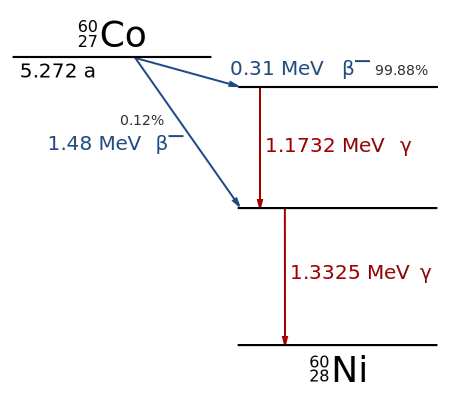
\includegraphics[width=.3\textwidth]{./img/co60_decay.pdf}
	\caption*{Source: \url{commons.wikimedia.org/wiki/File:Cobalt-60_Decay_Scheme.svg}}
	\caption[The decay cascade of \ce{^{60}Co}]{\textbf{The decay cascade of \ce{^{60}Co}} After decaying from a 5+ spin state to a 4+ spin state of \ce{^{60}Ni} by beta decay with a probability of \num{99.88}\%, two gamma rays of energies \SI{1.17}{\MeV} and \SI{1.33}{\MeV} are emitted, each inhibting a spin of 2+.}
	\label{fig:co60_cascade}
\end{figure}
When the nucleus emits two gamma rays in a cascade, as shown in \autoref{fig:co60_cascade}, the spatial angular distribution of the second photon with respect to the first photon's direction of travel is anisotropic.
In particular, by detecting two rays of a cascade simultaneously, the equal population of states is removed, resulting in an anisotropy of the second ray's angular distribution.
The relative probability of the gamma ray's emission at an angle $\theta$ relative to the first photon is denoted as $W(\theta)$.
Normalizing this differential cross-section at $\theta=\SI{90}{\degree}$ yields the correlation function

\begin{equation*}
	K(\theta) = 1 + \sum_{k}^{k_\text{max}}a_{2k}\cdot\cos^{2k}{\theta}.
\end{equation*}

The series terminates at $k_\text{max}=\min(I, L_1, L_2)=2$, where $I, L_1, L_2$ denote the nuclear spin after the first gamma emission and the angular momenta of both gamma rays respectively.
This results in the correlation function

\begin{equation}\label{eq:corr_func}
	K(\theta) = 1 + a_2\cos^{2}{\theta} + a_4\cos^{4}{\theta},
\end{equation}
while only pure multipole orders (quadrupoles) are assumed.

The deviation of a correlation function from an isotropic angular distribution is called \textbf{anisotropy}
\begin{equation}\label{eq:aniso}
	An=\frac{K(180)-K(90)}{K(90)}=K(180)-1
\end{equation}

\section{Resolution Time}
Utilizing the relation
\begin{equation}\label{eq:res_time}
	\tau_\text{res}=\frac{N_\text{R}}{N_1\cdot N_2}\cdot T,
\end{equation}
where $N_\text{R}$ denotes random event count, $N_{1/2}$ the number of events of channel 1/2 respectively and $T$ the length of the measurement, the resolution time of coincidences can be computed. \todo{Kinda bloated sentence. Any suggestions?}

\section{Detectors}
To not only being able to detect the mere presence of a gamma ray but also its energy, two \ce{NaI}-scintillators doped with \ce{Th} are employed.
Sodium iodide is an inorganic scintillator crystal and grants the advantage of most of the gamma rays being observed through the photoelectric effect.
Coupled to these scintillator crystals are two photomultiplier stages that output a voltage proportional to the incoming gamma ray's energy. \todo{Is it? i.e. non-linearity of crystals}
The output is digitized for later analysis.

	\chapter{Procedure}

\section{Geometry of the Setup}
\begin{figure}[tbp]
	\centering
	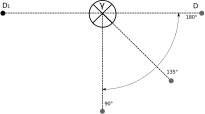
\includegraphics[width=0.5\textwidth]{./img/setup.pdf}
	\caption[Geometry of the Setup]{\textbf{Geometry of the Setup} Detector $D_2$ moves between angles 180, 135 and 90 degrees, while detector $D_1$ is at a fixed position and defines the quantization axis.}
	\label{fig:setup}
\end{figure}
The setup consists of two detectors, discussed in \autoref{sec:detectors}, centered around the $\gamma$-source, as can be seen in \autoref{fig:setup}.
As both detectors are located at a certain distance from the radiation source, the solid angle of detected radiation has to be accounted for in the analysis.
Unfortunately, these corrections are not the same for all measurement series, as the used construction's detector arms vary in distance.

\section{Measurement}
\begin{figure}[tbp]
	\centering
	\includegraphics[width=0.5\textwidth]{./data/plots/e-spectrum.pdf}
	\caption[First energy spectrum]{\textbf{First energy spectrum} Features a back-scatter peak, compton edge and two photo peaks corresponding to the observed decay cascade.}
	\label{fig:e_spectrum}
\end{figure}
To make sure both detector channels have the same energy scale and to determine a threshold, the spectrum of the first measurement is examined.
\autoref{fig:e_spectrum} shows this energy spectrum.
An energy threshold is necessary to filter out any lower energy random coincidences caused by Compton scattering and the like.
This threshold is set at channel number 3700, which roughly equals 60\% of the center point's energy between the photopeaks.
Six measurement series for 3 angles, each with an acquisition time of $T=\SI{320}{\second}$ are conducted.
One measurement with no active isotope is carried out to account for background radiation.

	\chapter{Data}
The gathered data will be evaluated using two different methods.
In the first method, all reduced event counts for each angle are added up and used for calculating coefficients $a_2$ and $a_4$,
whereas in the second method, the data is analyzed for each individual measurement series.

\section{False Coincidences}
Suppose two individual decays randomly happen at the same time, hence are not correlated.
Using the described detector setup would result into measuring a false coincidence.
To compensate for this, a time offset is applied to the measured event counts later on in the analysis.
This way, true coincidences are generally excluded and only false coincidences remain, which can be subtracted from the total measured coincidence counts.
\autoref{tab:data} shows measured false coincidences.

In the following, false coicidences are denoted with $N_\text{F}$.

\section{Background}\label{sec:bg}
Background radiation data can be seen in \autoref{tab:data}.
As data suggests, background radiation will not have a significant effect on the data as it is several orders of magnitude weaker than the examined effect.

Denoting background radiation counts with $N_\text{bg}$.

\section{Distance Correction}
As already mentioned in \autoref{sec:geom}, distance correction must be applied to the event counts.
In subsequent sections, distances will have been corrected already.

\section{Reduced Event Counts}
To account for temperature drifts and thresholds, all coincidence counts must be divided by their individual associated counts after backgrounds and false coincidences are subtracted
\begin{equation}\label{eq:red}
	R(\theta)=\frac{N_\text{c}-N_\text{cbg}-N_\text{F}}{(N_1-N_\text{bg})(N_2-N_\text{bg})}.
\end{equation}

Assuming a poisson distribution, the errors of event counts are their square root, which gives
\begin{align*}
	\sigma_\text{R} &= \sqrt{\left(\pdb{R}{N_\text{c}}\cdot\sigma_{N_\text{c}}\right)^2
	+ \left(\pdb{R}{N_\text{F}}\cdot\sigma_{N_\text{F}}\right)^2
	+ \left(\pdb{R}{N_1}\cdot\sigma_{N_2}\right)^2
	+ \left(\pdb{R}{N_2}\cdot\sigma_{N_2}\right)^2} \\
	&=\frac{1}{(N_1-N_\text{bg})(N_2-N_\text{bg})}
	\cdot\sqrt{N_\text{c} + N_\text{F} + \left(\frac{N_\text{c}-N_\text{F}}{N_1-N_\text{bg}}\right)^2\cdot N_1
	+ \left(\frac{N_\text{c}-N_\text{F}}{N_2-N_\text{bg}}\right)^2\cdot N_2},
\end{align*}
for the propagated error of reduced event counts, where background radiation is negligably small as discussed in \autoref{sec:bg}.

\section{Evaluation: Method One}
Adding all reduced event counts for each angle and propagating their corresponding errors like
\begin{equation*}
	\sigma_{R_\theta}=\sum_{i=1}^{6}\sigma_\text{R,i}^2,
\end{equation*}
where $i$ denotes the number of the measurement series, yields the values
\begin{itemize}
	\item $R_\theta (90)=\num{3.640(79)e-7}$
	\item $R_\theta (135)=\num{3.303(80)e-7}$
	\item $R_\theta (90)=\num{3.953(83)e-7}$
\end{itemize}
for the sum of reduced coincidences per angle.

Using formulae \ref{eq:A} and \ref{eq:B}, the auxiliary quantities $A$ and $B$ are calculated as
\begin{align*}
	A &= \num{0.907(30)} \\
	B &= \num{1.086(33)},
\end{align*}
while their corresponding errors propagate like
\begin{align}
	\sigma_\text{A} &= \sqrt{\left(\pdb{A}{R_\theta (90)}\cdot\sigma_{R_\theta(90)}\right)^2 + \left(\pdb{A}{R_\theta (135)}\cdot\sigma_{R_\theta(135)}\right)^2} \label{eq:err_A} \\
	\sigma_\text{B} &= \sqrt{\left(\pdb{B}{R_\theta (90)}\cdot\sigma_{R_\theta(90)}\right)^2 + \left(\pdb{B}{R_\theta (180)}\cdot\sigma_{R_\theta(180)}\right)^2}. \nonumber
\end{align}

Finally, the required correlation function coefficients and anisotropy can be calculated.
Utilizing equations \ref{eq:a2}, \ref{eq:a4} and \ref{eq:aniso} yields the values
\begin{alignat*}{3}
	a_2 &= \num{-0.456(123)} &&\Rightarrow \text{(relative deviation from theoretical value: 464.96\%)}\\
	a_4 &= \num{0.542(136)}  &&\Rightarrow \text{(relative deviation from theoretical value: 1200.87\%)} \\
	An  &= \num{0.086(33)}   &&\Rightarrow \text{(relative deviation from theoretical value: 48.61\%)},
\end{alignat*}
while their errors propagate like
\begin{align}
	\sigma_\text{$a_2$} &= \sqrt{\left(\pdb{a_2}{A}\cdot\sigma_\text{A}\right)^2 + \left(\pdb{a_2}{B}\cdot\sigma_\text{B}\right)^2} \label{eq:err_a}\\
	&=\sqrt{\left(4\cdot\sigma_\text{A} \right)^2 + \left(-1\cdot\sigma_\text{B} \right)^2} \nonumber\\
	\sigma_\text{$a_4$} &= \sqrt{\left(\pdb{a_4}{A}\cdot\sigma_\text{A}\right)^2 + \left(\pdb{a_4}{B}\cdot\sigma_\text{B}\right)^2}\nonumber \\
	&=\sqrt{\left(-4\cdot\sigma_\text{A} \right)^2 + \left(2\cdot\sigma_\text{B} \right)^2}\nonumber \\
	\sigma_\text{An} &= \sigma_\text{B}\nonumber.
\end{align}

\section{Evaluation: Method Two}\label{sec:meth_two_lel_i_said_meth}
\begin{table}[tbp]\small
	\centering
	\caption[Method Two: Coefficient Values]{\textbf{Method Two: Coeffcient Values} for each measurement series}
	\label{tab:aux_coeff}
	\begin{tabular}{cS[separate-uncertainty=false,table-format=1.2e-1]S[separate-uncertainty=false,table-format=1.2e-1]S[separate-uncertainty=false,table-format=1.2e-1]S[separate-uncertainty=false,table-format=1.2e-1]S[separate-uncertainty=false,table-format=1.2e-1]S[separate-uncertainty=false,table-format=1.2e-1]}
		\toprule
		{Run}& {$A_i$}& {$B_i$}& {$a_{2,i}$}& {$a_{4,i}$}& {$An_i$}\\
		\midrule
		1&0.822 \pm 0.067&	1.094 \pm 0.080&	-0.81 \pm 0.28&	-0.81 \pm 0.31&0.094 \pm 0.080\\
		2&1.006 \pm 0.082&	1.252 \pm 0.094&	-0.23 \pm 0.34&	-0.23 \pm 0.38&0.252 \pm 0.094\\
		3&0.872 \pm 0.070&	1.054 \pm 0.078&	-0.57 \pm 0.29&	-0.57 \pm 0.32&0.054 \pm 0.078\\
		4&0.851 \pm 0.070&	1.017 \pm 0.077&	-0.61 \pm 0.29&	-0.61 \pm 0.32&0.017 \pm 0.077\\
		5&0.902 \pm 0.071&	1.039 \pm 0.077&	-0.43 \pm 0.29&	-0.43 \pm 0.32&0.039 \pm 0.077\\
		6&1.003 \pm 0.075&	1.076 \pm 0.079&	-0.06 \pm 0.31&	-0.06 \pm 0.34&0.076 \pm 0.079\\
		\bottomrule
	\end{tabular}
\end{table}
Calculating the auxiliary coefficients $A$ and $B$ for each measurement series yields six individual values for these quantities.
Errors propagate in the same fashion as in \autoref{eq:err_A}.
Using these values, correlation function coefficients $a_2$, $a_4$ and anisotropy $An$ can be calculated, with error propagation as seen in \autoref{eq:err_a}.
All previously mentioned data can be seen in \autoref{tab:aux_coeff}.
Finally, the mean values of all quantities are computed.
Mean value formation over $N$ values generates a statistical error of
\begin{equation*}
	\sigma_\text{stat} = \frac{\sigma_\text{std}}{\sqrt{N}},
\end{equation*}
with standard deviation $\sigma_\text{std}$.
Additionally, the errors from previously calculated coefficients propagate into their mean value as
\begin{equation*}
	\sigma_\text{sys} = \sqrt{\frac{1}{N}\sum_{i=1}^N\sigma_\text{$a_2/a_4/An$}^2}.
\end{equation*}
However, these errors turn out to be negligable ($\approx\pm\num{0.363e-4}$).
Applying these deliberations yields the final values for the sought-after quantities
\begin{alignat*}{3}
 a_2 &= \num{-0.452}\pm\num{0.1010}\ \text{(stat.)} &&\Rightarrow \text{(relative deviation from theoretical value: 461.48\%)}\\
 a_4 &= \num{0.541}\pm\num{0.0935}\ \text{(stat.)}  &&\Rightarrow \text{(relative deviation from theoretical value: 1197.27\%)} \\
 An  &= \num{0.089}\pm\num{0.0315}\ \text{(stat.)}   &&\Rightarrow \text{(relative deviation from theoretical value: 46.90\%)},
\end{alignat*}

\section{Evaluation: Resolution Time}
Using formula \ref{eq:res_time} for each measurement, effectively generating $3\times 6 = 18$ values for $\tau$ and averaging these yields
\begin{equation*}
	\tau = (\num{106.15}\pm\num{72.15}\ \text{(sys.)}\pm \num{26.18}\ \text{(stat.)})\ \si{\ns}.
\end{equation*}
Errors for each value of tau propagate like
\begin{align*}
	\sigma_{\tau_i,\text{sys}} &= \sqrt{\left(\pdb{\tau}{N_\text{F}}\cdot\sigma_{N_\text{F}}\right)^2 + \left(\pdb{\tau}{N_1}\cdot\sigma_{N_1}\right)^2 + \left(\pdb{\tau}{N_2}\cdot\sigma_{N_2}\right)^2} \\
	&= \sqrt{ \left(\frac{T}{N_1\cdot N_2}\cdot\sigma_{N_\text{F}}\right)^2 + \left(-\frac{\tau}{N_1}\cdot\sigma_{N_1}\right)^2 + \left(-\frac{\tau}{N_2}\cdot\sigma_{N_2}\right)^2}
\end{align*}
and finally, by averaging, the systematic error propagates like
\begin{equation*}
	\sigma_{\tau,\text{sys}} = \sqrt{\frac{1}{18}\sum_{i=1}^{18}\sigma_{\tau_i,\text{sys}}^2}.
\end{equation*}
Additionally, averaging generates a statistical error of
\begin{equation*}
	\sigma_{\tau,\text{stat}} = \frac{\sigma_{\tau,\text{std}}}{\sqrt{18}},
\end{equation*}
just as in \autoref{sec:meth_two_lel_i_said_meth}.

	\chapter{Results}
The experiment does not confirm the theory.
In general, the literature values do not lie within their respective error boundaries.
Both methods approximately yield the same error limits and values.
The considered errors turn out to be large in relation to their values.
However, keeping in mind that the error limits in method two can be minimized with increasing measurement time and series, one can obtain better certainty on the quantities to be determined.

The fact that all established quantities do not resemble their respective literature values suggests two possible explanations:
Either the experiment was performed incorrectly, or the used equipment is faulty.
Considering \autoref{fig:e_spectrum}, one might notice the indistinct peaks and blurred slopes in the energy spectrum, which encourages the assumption that the second explanation might be more likely to be true.\todo{Just looking for excuses... :D}

The experiment can be improved by increasing the measurement time and checking the equipment.

	\Appendix
\configureappendix

	%\TheBibliography
\bibliographystyle{babalpha}
\bibliography{../common/lit}

\end{document}
